\documentclass[pdf]{beamer}
\mode<presentation>{\usetheme{Warsaw}}
\usepackage{amssymb, amsmath}
\usepackage{graphicx}
\usecolortheme{dolphin}
\useinnertheme{rounded}
\useoutertheme{smoothbars}

\title{Computational Methods in Statistics I}
\subtitle{Dimension Reduction: An Application In Facial Recognition} 
\author{Joe Sinotte}
\begin{document}

\begin{frame}
\titlepage
\end{frame}

\section{Introduction}
\begin{frame}{Outline}
\begin{itemize}
\item Motivation and Statement of the Problem
\item Methodology
\begin{itemize}
\item PCA
\item SP
\end{itemize}
\item Results
\item Conclusion
\end{itemize}
\end{frame}                                                                                                                                                                                                                                                                                                                                                                                                                                                                                                                                                                                                                                                                                                                                                                                                                                                                                                                                                                                                                                                                                                                                                                                                                                                                                                                                                                                                                                                                                                                                                                                                                                                                                                                                                                                                                                                                                                                                                                                                                                                                                                                                                                                                                                                                                                                                                                                                                                                                                                                                                                                                                                                                                                                                                                                                                                                                                                                                                                                                                                                                                                                                                                                                                                                                                                                                                                                                                                                                                                                                                                                                                                                                                                                                                                                                                                                                                                                                                                                                                                                                                                                                                                                                                                                     
                                                                                                                                                                                                                                                                                                                                                                                                                                                                                                                                                                                                                                                                                                                                                                                                                                                                                                         
\begin{frame}{Motivation}
\begin{itemize}
\item Image recognition is widely used in the world today.
\begin{itemize}
\item Law Enforcement
\item Mapping
\item Social Media
\end{itemize}
\item Thus, the ability to correctly perform image recognition is applicable in many fields of study.
\end{itemize}
\end{frame}

\begin{frame}{Statement of the Problem}
Data:
\begin{itemize}
\item two sets of 200 images taken of 40 individuals.
\item each individual has five different images in each set.
\end{itemize}
Problem: Given the data, can a program be written to correctly match an image from one set to a person in the other set?
\end{frame}

\section{Methodology}
\begin{frame}{Dimension Reduction}
\begin{itemize}
\item Data sets for images are often quite large.
\item It is often convenient to use transformations to reduce the dimensionality of the images.
\item Two methods of dimension reduction will be used:
\begin{itemize}
\item PCA
\item SP
\end{itemize}
\end{itemize}
\end{frame}

\begin{frame}{Principal Component Analysis}
\begin{itemize}
\item The data set is multiplied by the transpose of the first K columns of an orthogonal matrix found by using Singular Value Decomposition.
\item This method allows the user to choose the number of dimensions that give the most descriptive information of the data. The superfluous data are eliminated from the rest of the application.
\end{itemize} 
\end{frame}

\begin{frame}{Simple Projection}
\begin{itemize}
\item The matrix used to transform the data is derived by selecting the first K columns of an identity matrix which, in this example, is of dimension $(s_{1} \times s_{2})=644$.
\item The data are then transformed by premultiplying Ytest and Ytrain by the transpose of this matrix.
\end{itemize}
\end{frame}

\begin{frame}{Nearest Neighbor}
\begin{itemize}
\item A column (image) was selected at random from Ytest, with the goal being to find a match in Ytrain.
\item The Nearest Neighbor Classifier was used to find the match, where the NN is the image in Ytrain that minimizes the normed distance between itself and the column of Ytest. 
\item The matching is successful if the two images correspond to the same individual.
\end{itemize}
\end{frame}

\section{Results}
\begin{frame}{Match with SP}
Here is an example of a match using the Simple Projection Method:
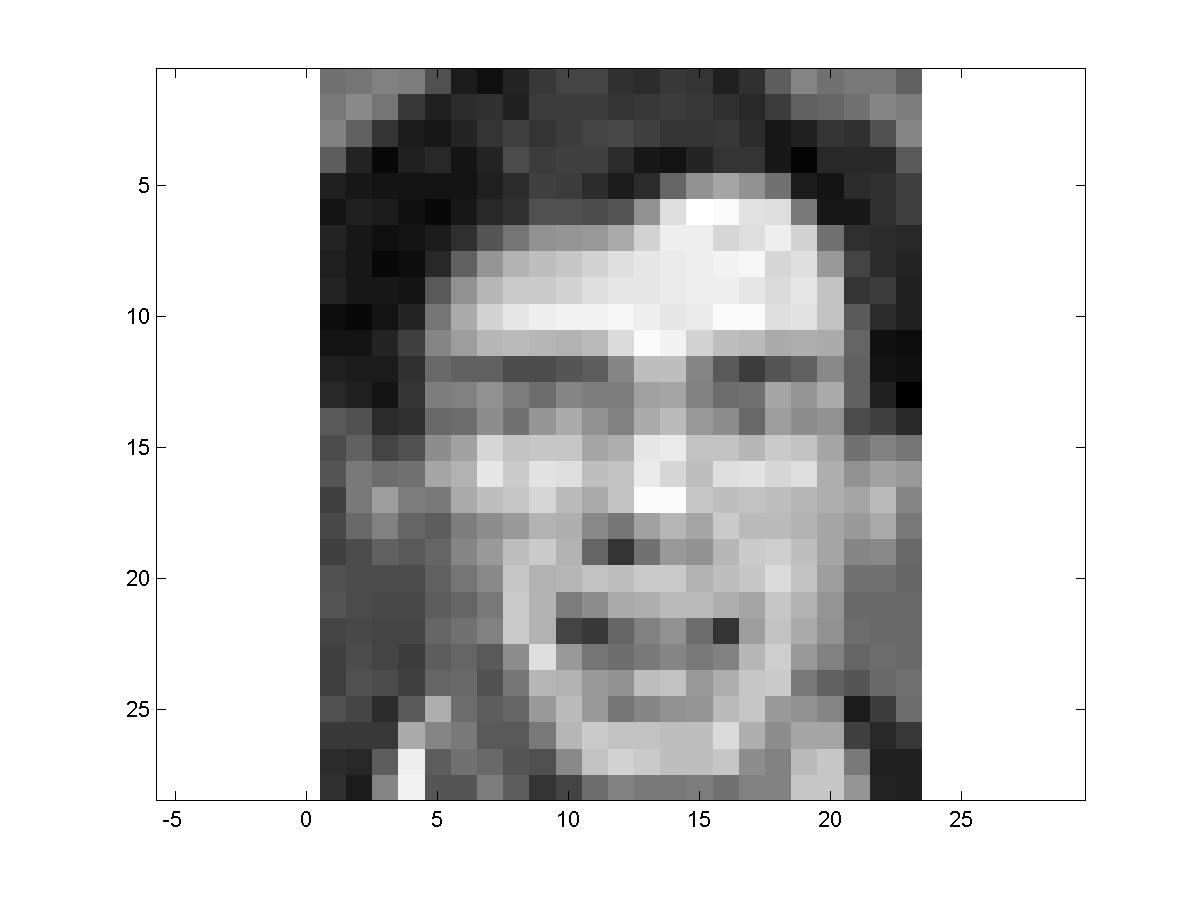
\includegraphics[scale=.13]{figure2}
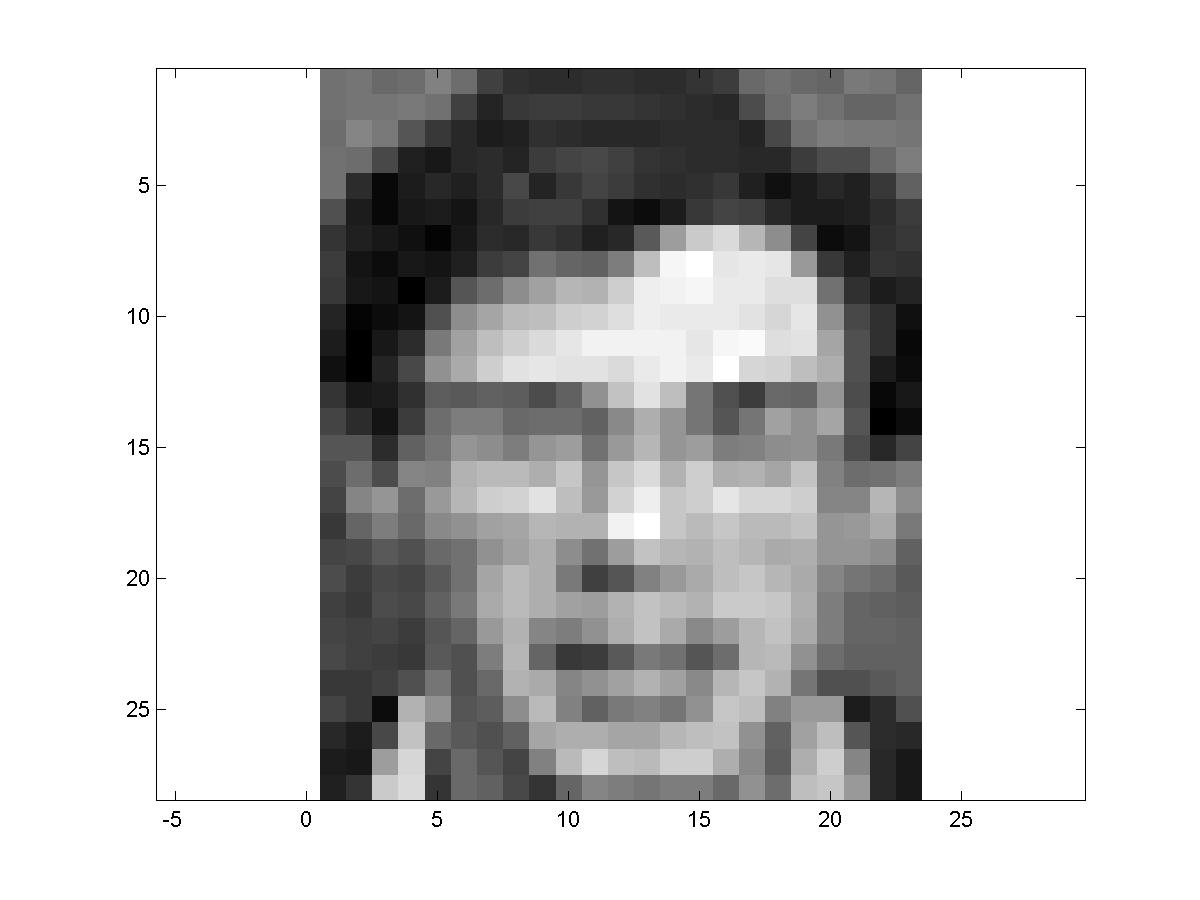
\includegraphics[scale=.13]{figure3}
\end{frame}

\begin{frame}{Match with PCA}
Here is an example of a match using the Pricinpal Component Analysis:
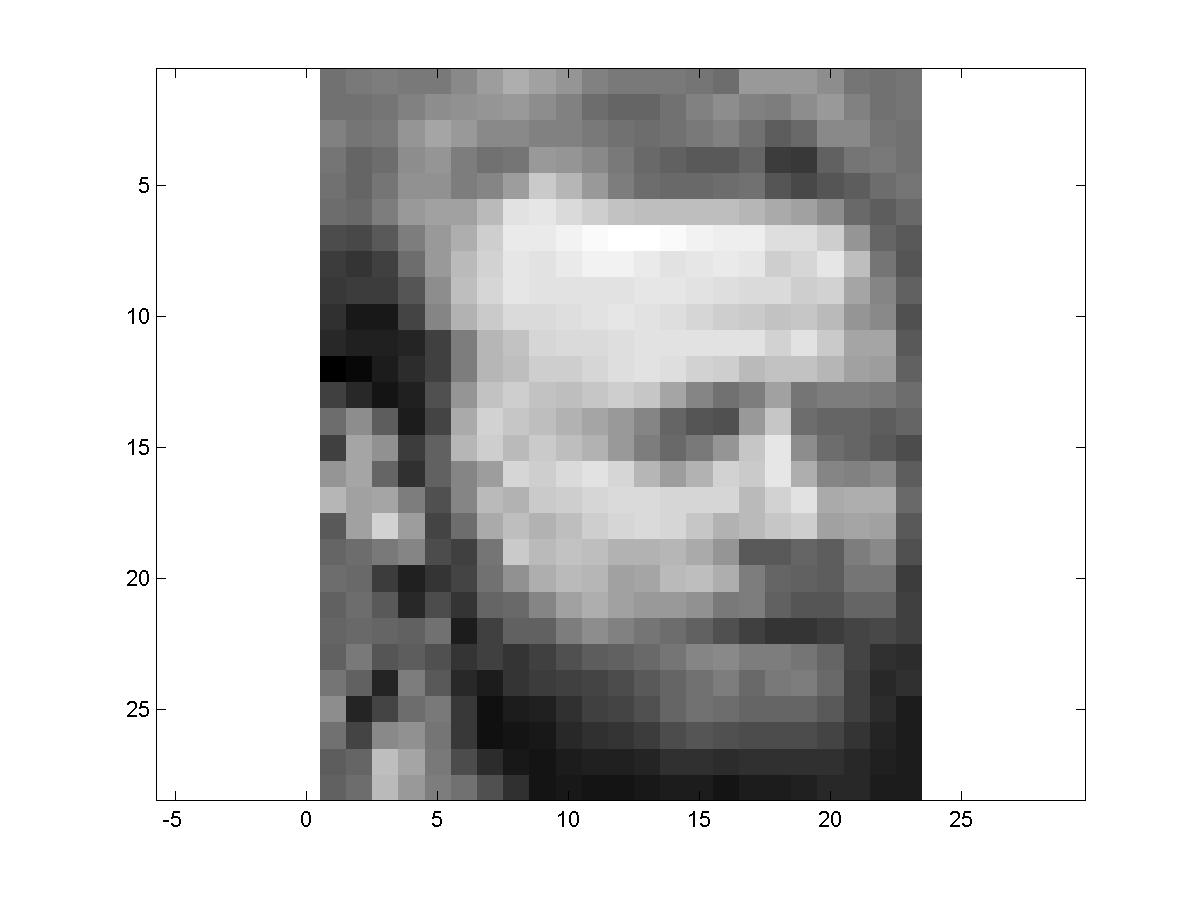
\includegraphics[scale=.13]{figure4}
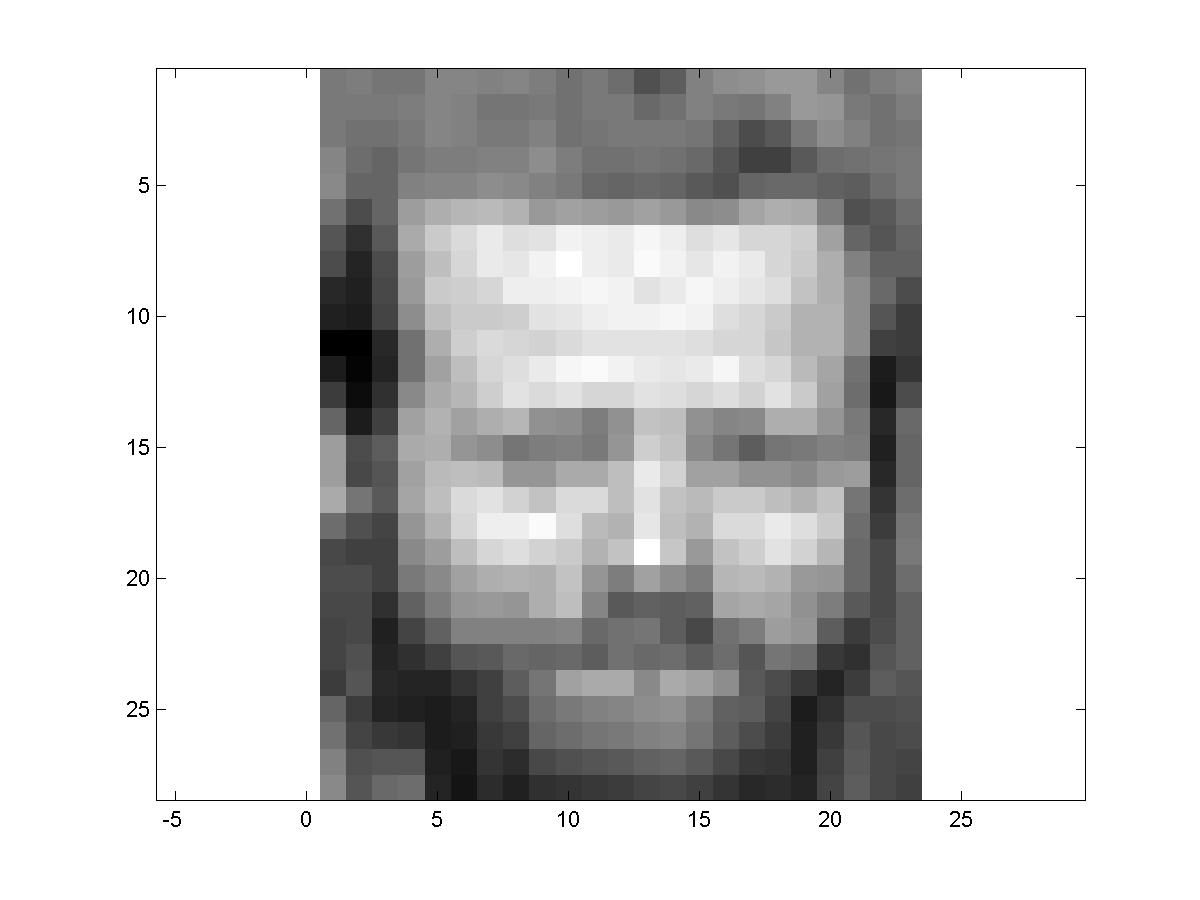
\includegraphics[scale=.13]{figure5}
\end{frame}

\begin{frame}{Results}
\begin{center}
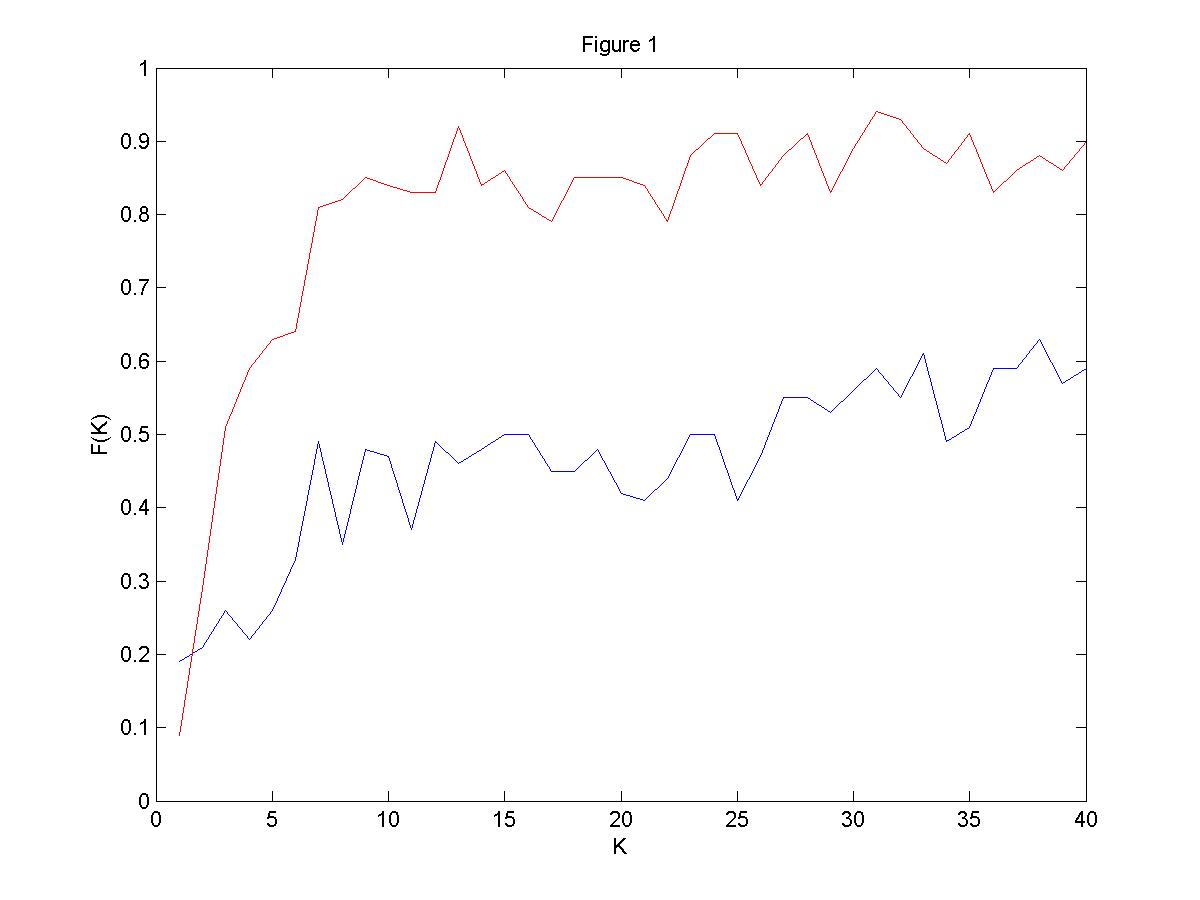
\includegraphics[scale=.22]{figure1}
\end{center}
\end{frame}

\section{Conclusions}
\begin{frame}{Conclusions}
\begin{itemize}
\item Overall, the exercise is a success.
\item SP is better for small dimensional data.
\item With larger dimensional data sets, PCA becomes much more accurate than SP.
\end{itemize}
\end{frame}
\end{document}